%! Author = itgramic
%! Date = 05.12.23

% Preamble
\clearpage
\begin{flushleft}
    \subsubsection{Patroni}
    Patroni ist eine von Zalando auf Basis von Python entwickelte HA-Lösung für \Gls{PostgreSQL}.\\
    Patroni wird aktiv von Zalando gepflegt.
\end{flushleft}
\begin{flushleft}
    \paragraph{Core-Features}
    Patroni bietet folgende Core-Features:
    \begin{itemize}
        \item Rest-API und eigenes Skript- und Toolset
        \item Aktionen und Konfigurationen im Konsensprinzip abgestimmt
        \item Manueller oder Sheduled Switchover
        \item Reines PostgreSQL als Basis, Patroni setzt Hilfe von Python darauf auf
        \item Automatische reintegration von Nodes nach einem Fehler
        \item Citus kompatibel
        \item Docker und Docker-compose Dokumentation
    \end{itemize}
\end{flushleft}
\begin{flushleft}
    \paragraph{Replikation}
    Patroni bietet per Default eine eigene Replikation an.\\
    Diese ist allerdings eine asynchrone Replikation.
\begin{flushleft}
    Patroni unterstützt aber die synchrone Replikation von \Gls{PostgreSQL}.
\end{flushleft}
\end{flushleft}
\begin{flushleft}
    \paragraph{Proxy}
    Patroni benötigt einen \Gls{HAProxy}, um Load Balancing betreiben zu können\cite{VYXTI7BS}.
\end{flushleft}
\begin{flushleft}
    \paragraph{Pooling}
    Patroni benötigt einen externen \Gls{Connection Pooler}.\\
    Hier wird oft PgBouncer \cite{ATBELZ2X} verwendet.
\end{flushleft}
\begin{flushleft}
    \paragraph{API / Skripte}
    Patroni hat ein eigenes Tool- und Commandset, \texttt{patronictl}, welches die Verwaltung vereinfacht.\\
    Es umfasst das Ändern und Erfassen von Konfigurationen, das Forcieren eines Failovers als Switchover, Maintenance Handling und Informationsbeschaffung.\\
    Zusätzlich bietet Patroni eine API, welche Daten für das Monitoring bereitstellt,\\
    aber auch Betriebsfunktionen zur Verfügung stellt.\\
\end{flushleft}
\begin{flushleft}
    \paragraph{\gls{etcd}}
    Patroni benötigt etcd oder \Gls{Consul} als \Gls{Key-Value-Store}.
\end{flushleft}
\begin{flushleft}
    \paragraph{Architektur}
    Das Architektur-Schaubild sieht folgendermassen aus:
    \begin{figure}[H]
        \centering
        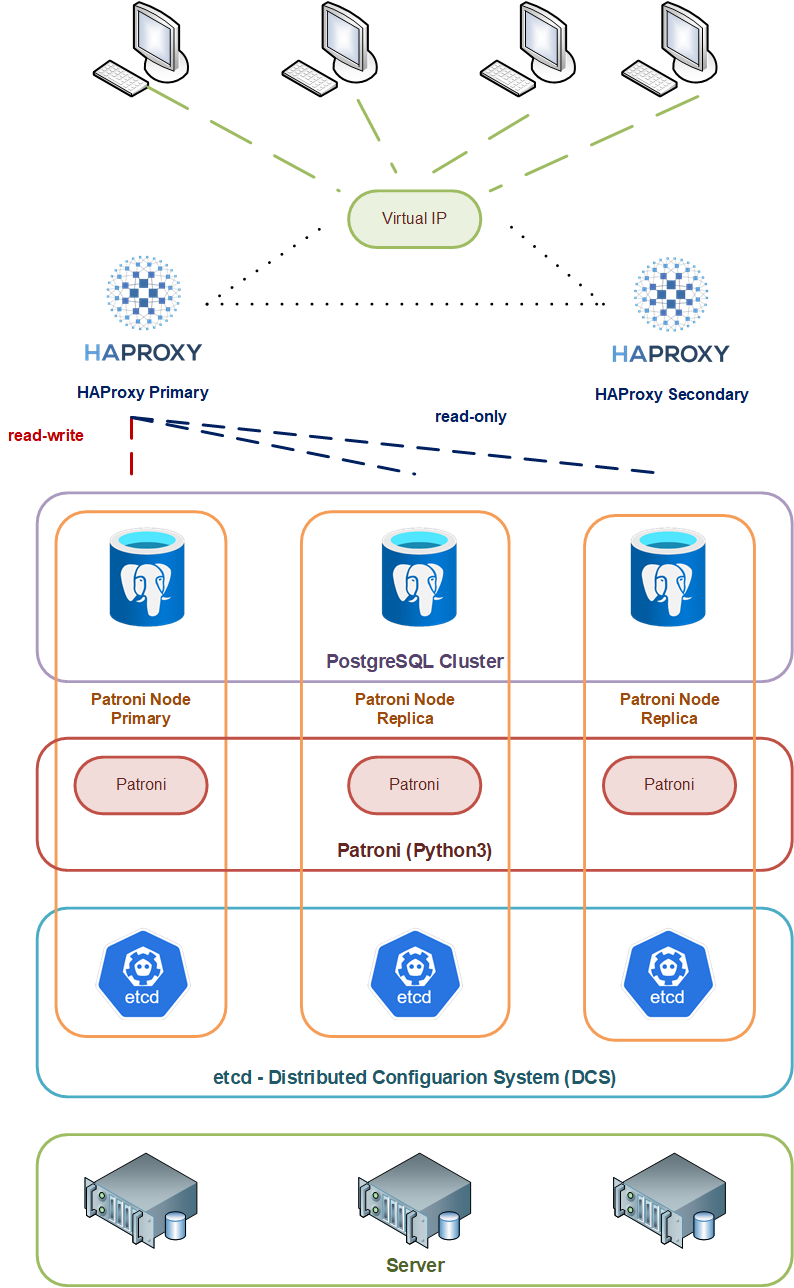
\includegraphics[width=0.7\linewidth]{source/implementation/evaluation/postgresql_ha_solutions/patroni_architecture}
        \caption{Patroni-Architektur}
        \label{fig:patroni-architecture}
    \end{figure}
\end{flushleft}
\begin{flushleft}
    \paragraph{Maintenance}
    Patroni ist ein sehr gepflegtes Projekt, welches die gängigen Community Standards einhält.\\
    Die Details sind im \hyperref[subsec:maintenance_patroni]{Anhang - Maintenance} zu finden.
\end{flushleft}
\begin{flushleft}
    \paragraph{Synergien und Mehrwert}
    Patroni kann nicht nur mit Citus zu einem Distributed / Sharded SQL System umgebaut werden,\\
    es ist auch Kern von StackGres.
\end{flushleft}
\begin{flushleft}
    Damit könnten die API und Skripte in beiden Welten verwendet werden.\\
    Der Aufwand für die Verwaltung und Optimierung würde stark gesenkt.\\
    Projekte wie \texttt{vitabaks / postgresql\_cluster}\cite{HIQVBEPF} bieten zudem die Vorlage für eine noch stärkere Automatisierung.
\end{flushleft}